\section{Question 3}

\begin{question}
   $\left\{\begin{array}{l}u_t+u_x=0, \quad t>0, \quad x \in(0,1) \\ u(x, 0)=-\sin (3 \pi x), \text{ if } x \in\left[0, \frac{1}{3}\right) ; \; 1 \text { if } x \in\left[\frac{1}{3}, \frac{2}{3}\right) ; \; 0 \text{ if } x \in\left[\frac{2}{3}, 1\right] \\ u(0, t)=u(1, t), \quad t>0 .\end{array}\right.$
   
    Compute the solution at $t=10$ with at least 6 methods. Plot your numerical solutions against the exact solution at $t=10$.
\end{question}

\begin{answer}
    I used implemented the Center Difference Scheme, Up Wind Scheme, Lax-Friedrichs Scheme, Lax-Wendroff Scheme, Beam-Warming Scheme, and MacCormack Scheme to compute the solution at $t = 10$ in $\MATLAB$, and I plot the solutions and the exact solution at $t = 10$ in the Figure \ref{fig:fig1}.
    \begin{figure}[H]
        \centering
        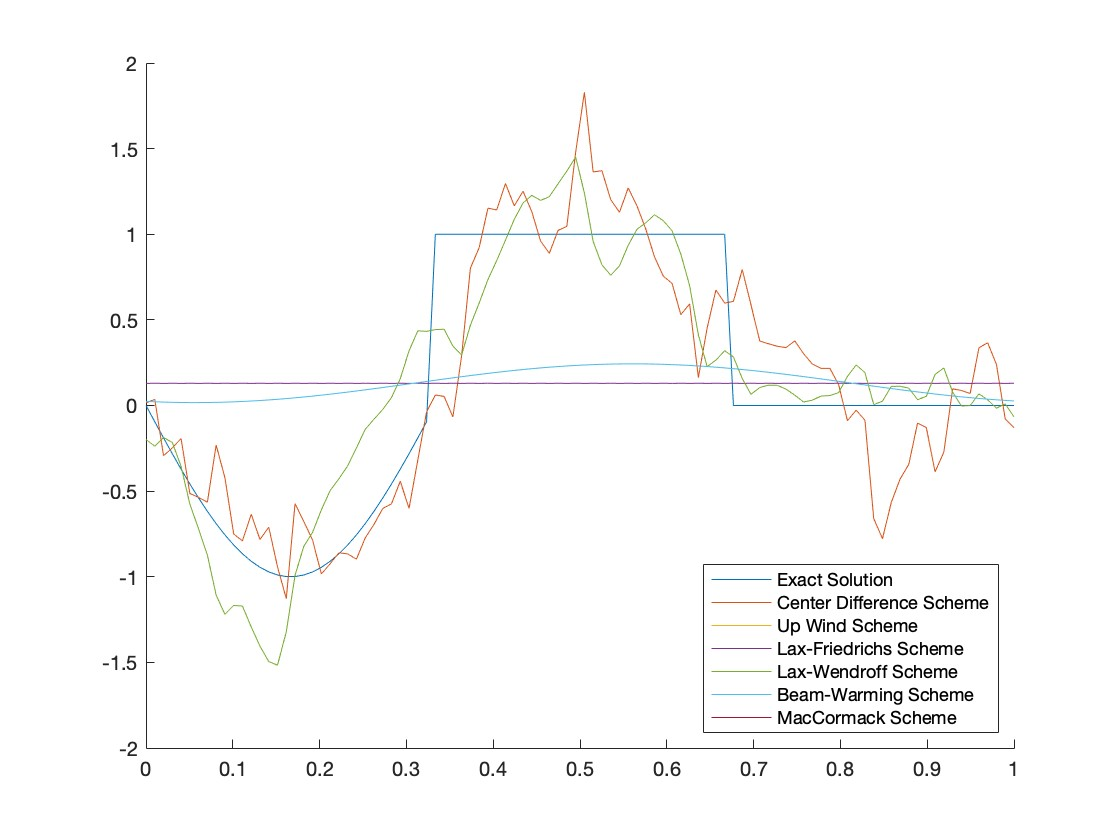
\includegraphics[width=0.99\textwidth]{Result.jpg}
        \caption{\label{fig:fig1}Numerical Results}
    \end{figure}
\end{answer}